\documentclass[output=paper]{langsci/langscibook}
\ChapterDOI{10.5281/zenodo.3972834}

\author{Robert D. Borsley\affiliation{University of Essex and Bangor University}}
\title{Comparative syntax: An HPSG perspective}

% \chapterDOI{} %will be filled in at production

\abstract{There has been little explicit discussion of comparative matters in
    the HPSG literature, but HPSG has a number of properties which make it
    relevant to comparative syntax. Firstly, it emphasizes detailed formal
    analyses, often incorporated into a computer implementation. This means
    that the framework provides firmer foundations than some other approaches
    for claims about individual languages and about language in general.
    Secondly, it stresses how little is really known about what is and is not
    possible in natural language syntax. Thirdly, it seeks to develop concrete
    analyses closely linked to the observable data, which keep the
    acquisition\is{language acquisition} task as simple as possible and create
    as little need as possible for innate apparatus. These properties suggest
    that HPSG can make an important contribution to the comparative syntax.}

\maketitle

\begin{document}\glsresetall

\section{Introduction}

In what ways are languages alike in their syntax? In what ways can they differ?
Comparative syntax seeks to answer these questions and perhaps to explain the
answers that it arrives at. It has been a major focus of \gls{MGG}\footnote{I
    take this term from \citet{CulJac2005}, who define it as \enquote{the line
    research most closely associated with Noam Chomsky} (fn.\ 1, p.\ 3). It refers
    to a variety of different but related approaches. Like
    \citeauthor{CulJac2005} I do not regard \enquote{mainstream} as a synonym for
\enquote{correct}.} since the emergence of the Principles and Parameters framework in
the early 80s, and it has been a central concern of Ian Roberts \parencite[see
e.g.][]{Roberts1997,Roberts2007}. However, the questions that define the field
of comparative syntax are of interest not just to \gls{MGG} but to any serious
approach to syntax. In this paper, I will consider what the \gls{HPSG}
framework can say about them. Although there has been work in \gls{HPSG}\is{Head-Driven Phrase Structure Grammar} on a
variety of languages, there has not been much explicit discussion of
comparative matters in the main \gls{HPSG}\is{Head-Driven Phrase Structure Grammar} literature. Typical papers say
\enquote{here is a good way to deal with phenomenon P in language L} and not
\enquote{here’s an interesting way in which languages may differ}. However, it
is not too hard to spell out a view of comparative matters that is implicit in
much \gls{HPSG}\is{Head-Driven Phrase Structure Grammar} work.  Moreover, \gls{HPSG}-based computational work has often
been concerned with comparative issues, in particular with developing minimally
different grammars for a variety of languages (see e.g.~\citealt{Muller2015};
\citealt{BenDreFokPouSal2010,Bender2016}), and this work is also of some relevance
here. \gls{HPSG}\is{Head-Driven Phrase Structure Grammar} brings a number of ideas to the discussion of comparative
syntax. One is a stress on the importance of firm empirical foundations in the
form of detailed formal analyses. Another is an emphasis on how little we
really know about what is and is not possible in natural language syntax. A
third is an emphasis on the importance of developing concrete analyses which
keep the acquisition\is{language acquisition} task as simple as possible. I will discuss all of these in
the following pages.\is{HPSG|see{Head-Driven Phrase Structure Grammar}}

The paper is organized as follows. In~\Cref{sec-5:2}, I look at the Principles
and Parameters approach to comparative syntax and explain why proponents of
\gls{HPSG} are sceptical about it. Then in \Cref{sec-5:3}, I explain the main
components of \gls{HPSG}\is{Head-Driven Phrase Structure Grammar} grammars: types, features, and constraints. In
\Cref{sec-5:4}, I discuss the ways in which \gls{HPSG}\is{Head-Driven Phrase Structure Grammar} grammars may differ, and
in \Cref{sec-5:5}, I pull together the main ideas about comparative syntax that
I have introduced in the preceding sections. In \Cref{sec-5:conclusions} I
conclude the paper.

\section{Principles and parameters}\label{sec-5:2}

For \gls{MGG}, the ways in which languages are alike and the ways in which they
may differ are a reflection of an innate language faculty. The properties they
share are the result of innate principles, while the ways in which they may
differ are defined by innate \isi{parameters}. This position has been hugely
influential over the last 25 years. However, it seems fair to say that these
ideas, especially the idea of innate \isi{parameters}, have not been as successful as
was hoped when they were first introduced in the early 1980s.\footnote{See
\citet{Newmeyer2005} and \citet{Haspelmath2008} for relevant discussion.}

Outsiders have always been sceptical about these ideas. Thus,
\citet[31]{PolSag1994}, after considering the possibility of incorporating
parameters into \gls{HPSG}\is{Head-Driven Phrase Structure Grammar}, comment as
follows:

\blockquote{In the absence of a list, however tentative, of posited
    \isi{parameters} and their range of settings, together with a substantial,
    worked-out fragment for at least one language, a specification of the
    settings for that language, and a reasonably detailed account of how those
settings account for the array of facts covered in the fragment, we are
inclined to view parameter-based accounts of cross-linguistic variation as
highly speculative.}
%
More recently, linguists who are less obviously outsiders have come to similar
conclusions. Thus, \citet[75]{Newmeyer2005} writes as follows:

\blockquote{[\dots{}] empirical reality, as I see it, dictates that the hopeful
    vision of UG as providing a small number of principles each admitting of a
    small number of parameter settings is simply not workable. The variation
    that one finds among grammars is far too complex for such a vision to be
realized.}
%
At least one Minimalist has come to much the same conclusion.
\citet{Boeckx2011b} suggests that:

\begin{quote}

some of the most deeply-embedded tenets of the Principles-and-Parameters
approach, and in particular the idea of Parameter, have outlived their
usefulness.

\end{quote}

A major reason for scepticism about \isi{parameters} is that estimates of how many
there are seem to have steadily increased. \citet{Fodor2001} considers that
there might be just twenty \isi{parameters}, so that acquiring a grammatical system
is a matter of answering twenty questions. \citet[44]{Newmeyer2005} remarks
that \enquote{I have never seen any estimate of the number of binary-valued
    \isi{parameters} needed to capture all of the possibilities of core grammar that
    exceeded a few dozen}. However, \citet{RobHol2006} comment that
    \enquote{[n]early all estimates of the number of \isi{parameters} in the
    literature judge the correct figure to be in the region of 50--100}.
    Clearly, a hundred is a lot more than twenty. This is worrying. As
    \citet[6]{Newmeyer2006} observes, \blockquote{it is an ABC of scientific
        investigation that if a theory is on the right track, then its overall
        complexity decreases with time as more and more problematic data fall
    within its scope. Just the opposite has happened with parametric theory.
Year after year more new \isi{parameters} are proposed, with no compensatory decrease
in the number of previously proposed ones}.

The increasing numbers might not be a cause for concern if \isi{parameters} were just
seen as observations about how languages may vary, but if they are seen as part
of an innate language faculty, it is worrying. It is just not clear how there
could be so much that is innate. Moreover, a large number of innate \isi{parameters}
seems incompatible with the minimal conception of the language faculty that
Chomsky has championed over the last decade or so.\footnote{For further
discussion of \isi{parameters} and the problems they face, see \citet{Newmeyer2017}.}

Scepticism about \isi{parameters} is not a matter of saying that anything goes.  It
is also not a matter of rejecting any notion of an innate language faculty.
After all, Chomsky argued for a language faculty for two decades before he
formulated the idea of \isi{parameters}, and there are more recent advocates of a
language faculty who do not assume \isi{parameters}, for example \citet{CulJac2005}.
Thus, one might reject the idea of \isi{parameters} but still subscribe to the idea
of an innate language faculty.  However, neither evidence that there are
universal properties of language nor evidence that variation is limited is
necessarily evidence for an innate language faculty since there may be other
explanations. Thus, \citet[478]{Sag1997}, echoing much earlier work, suggests
that \enquote{\dots{} perhaps much of the nature of grammars can be explained
    in terms of general cognitive principles, rather than idiosyncratic
    assumptions about the nature of the human language faculty}. In rather
    similar vein, \citet[9]{Chomsky2005} advocates \enquote{\dots shifting the
        burden of explanation from the first factor, the genetic endowment, to
        the third factor, language-independent principles of data processing,
    structural architecture, and computational efficiency}.

Probably most proponents of \gls{HPSG}\is{Head-Driven Phrase Structure Grammar} would remain agnostic about these matters. No
doubt there are language universals and languages do not vary without limit, as
Joos suggested. But most \gls{HPSG}\is{Head-Driven Phrase Structure Grammar} linguists would think that we do not have enough
detailed formal analyses of enough phenomena in enough languages to have any
firm conclusions about these matters. In the absence of such conclusions, it is
not possible to say much about contributions of general cognitive principles
and purely linguistic principles to grammatical phenomena.

\section{The HPSG framework}\label{sec-5:3}

\gls{HPSG} emerged in the mid 1980s, building in various ways on earlier work,
and it has since been employed in theoretical and computational work on a
variety of languages.\footnote{As a referee has pointed out to me, many of the
    properties of \gls{HPSG}\is{Head-Driven Phrase Structure Grammar} that I highlight here are also features of Lexical
Functional Grammar.} It is a monostratal, constraint-based approach to syntax.
As a monostratal approach, it assumes that linguistic expressions have a single
constituent structure. This means that no constituent ever appears anywhere
other than its superficial position and hence that it has nothing like the
movement processes that are a feature of all versions of transformational
grammar. The relations that are attributed to \isi{movement} in transformational work
are captured by constraints that require certain features to have the same
value. For example, a \isi{raising} sentence is one with a verb which has the same
value for the feature \textsc{subj(ect)} as its complement. As a constraint-based
approach, it assumes that grammars involve sets of constraints, and a
linguistic expression is well-formed if and only if it conforms to all relevant
constraints. There are no procedures modifying representations such as the
Merge and \isi{Agree} operations of Minimalism. For arguments in favour of such a
declarative view of grammar, see e.g. \citet{PulScho2001}, \citet{Postal2003}
and \textcite{SagWas2011,SagWas2015}.

\gls{HPSG} is also a framework which places considerable emphasis on detailed
formal analyses of phenomena. Thus, it is not uncommon to find lengthy
appendices setting out formal analyses. See, for example, \citegen{Sag1997}
paper on \ili{English} \isi{relative clauses} and especially \citet{GinSag2000}, which has
a 50 page appendix. One consequence of this, alluded to above, is that
\gls{HPSG} has had considerable influence in computational linguistics.

A further important feature of \gls{HPSG}\is{Head-Driven Phrase Structure Grammar} is that it avoids abstract analyses
with tenuous links to the observable data. Phonologically empty elements are
only assumed if there is compelling evidence for them.\footnote{There may be
    compelling evidence for some empty elements in some languages. Thus,
    \textcite[Sec.\ 8]{Borsley2009} argues that \ili{Welsh} has phonologically empty
pronouns. For general discussion of empty elements, see \textcite[Sec.\
19.2]{Muller2016}.} Thus, the fact that some \ili{English} subordinate clauses
contain a complementizer\is{complementizers} is not seen as evidence that there is a phonologically
empty complementizer\is{complementizers} in subordinate clauses in which no complementizer\is{complementizers} is
visible. Similarly, overt elements are only assumed to have properties for
which there is clear evidence.  The fact that many languages have a case system
of some kind or some form of subject-verb agreement\is{agreement!subject
agreement} does not mean that they all do. This feature of HPSG stems largely
from considerations about acquisition\is{language acquisition}.  Every element or property which is
postulated for which there is no clear evidence in the data increases the
complexity of the acquisition\is{language acquisition} task and hence necessitates more complex innate
machinery. This suggests that such elements and properties should be avoided as
much as possible. It has important implications both for the analysis of
individual languages and for how we see differences between
languages.\largerpage[-3]

For \gls{HPSG}\is{Head-Driven Phrase Structure Grammar}, a linguistic analysis
is a system of types, features, and constraints.\footnote{The related but
    slightly different framework, Sign-Based Construction Grammar, has a
    further major element, namely constructions.\glsunset{SBCG} For \gls{SBCG}
    signs are defined in terms of constraints on constructions, whereas
    standard \gls{HPSG}\is{Head-Driven Phrase Structure Grammar} has
    constraints applying directly to signs. \gls{SBCG} is more complex in some
    respects but simpler in others. In particular, it has a simpler notion of
    sign and is able to dispense with a number of features and types which are
    assumed in \gls{HPSG}. See \textcite{Sag2010,Sag2012} for discussion.}
    Types provide a complex classification of linguistic objects, features
    identify their basic properties, and constraints impose further
    restrictions. The central focus of \gls{HPSG}\is{Head-Driven Phrase
        Structure Grammar} is signs.  For \citet{GinSag2000}, the type
        \emph{sign} has the subtypes \emph{lexical-sign} and \emph{phrase}, and
        \emph{lexical-sign} has the subtypes \emph{lexeme} and \emph{word}.
        Thus, we have the following type hierarchy:

\ea\label{ex-5:borsley:1}
    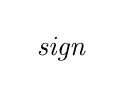
\begin{tikzpicture}[baseline=(root.base)]

        \Tree 	[.\node(root){\emph{sign}};
                    [.\emph{lexical-sign}
                        \emph{lexeme}
                        \emph{word}
                    ]
                    \emph{phrase}
                ]

    \end{tikzpicture}
\z
%
Both \emph{lexeme}   and \emph{phrase} have a complex system of subtypes.
In both cases, complex hierarchies mean that the framework is able to deal with
broad, general facts, very idiosyncratic facts, and everything in between. I
will say more about this below.

There are many other kinds of type. For example, there are types that are the
value of fairly traditional features like \textsc{person}, \textsc{number}, \textsc{gender}, and \textsc{case}. A
simple treatment of person might have the types \emph{first},
\emph{second}, and \emph{third}, and a simple treatment of number the types
\emph{sing}(\emph{ular}) and \emph{plur}(\emph{al}).\footnote{
\textrm{In practice a more complex system of values may well be appropriate.}}
Unlike the types mentioned above, these are atomic types with no features.
There are also types that provide the value of various less familiar features.
For example, \gls{HPSG}\is{Head-Driven Phrase Structure Grammar} has a feature \textsc{head}, whose value is a \emph{part-of-speech},
a type which indicates the part of speech of a sign and provides appropriate
information, e.g. information about person, number, gender, and case in the
case of nominal signs or finiteness in the case of verbal signs. Two other
important features are \textsc{subj(ect)} and \textsc{comp(lement)s}, whose value is a list of
\emph{synsem} objects, combinations of syntactic and semantic information.
The former, mentioned earlier, indicates what kind of subject a sign requires
and the latter indicates what complements it takes. Obviously, there are plenty
of opportunities here for languages to do things differently.

The type \emph{lexeme} and its subtypes and the associated constraints are the
core of the lexicon. In much \gls{HPSG}\is{Head-Driven Phrase Structure Grammar} work \emph{lexeme} has two distinct
sets of subtypes, one dealing with part-of-speech information and one dealing
with argument selection information. Here is a simple illustration based on
\citet[20]{GinSag2000}:

\ea\label{ex:borsley:4.2}
    \begin{tikzpicture}[baseline=(lex.base)]

        \tikzset{level 1/.style={sibling distance=50pt}}

        \Tree 	[.\node(lex){\emph{lexeme}};
                    [.\textsc{part-of-speech}
                        \node (v-lx) {\emph{v-lx}};
                        \dots{}
                        \dots{}
                        \dots{}
                    ]
                    [.\textsc{arg-selection}
                        [.\emph{intr-lx}
                            \node (s-rsg-lx) {\emph{s-rsg-lx}};
                            \dots{}
                            \dots{}
                        ]
                        \dots{}
                    ]
                ]

            \node [below=3.5cm of lex] (srv-lx) {\emph{srv-lx}};
            \draw (v-lx.south) to (srv-lx.north);
            \draw (s-rsg-lx.south) to (srv-lx.north);

    \end{tikzpicture}
\z
%
Upper case letters are used for the two dimensions of classification, and \emph{v-lx}, \emph{intr-lx}, \emph{s-rsg-lx}, and \emph{srv-lx} abbreviate \emph{verb-lexeme}, \emph{intransitive-lexeme}, \emph{subject-raising-lexeme}, and \emph{subject-raising-verb-lexeme}, respectively. All these types will be subject to specific constraints. For example, \emph{v-lx} will be subject to something like the following constraint:

\ea\label{ex:borsley:4.3}
    \emph{v-lx} → \avm[style=narrow]{
                        [head & verb\\
                         subj & < xp >]
                    }
\z
%
This says that a verb lexeme has a verbal part of speech and requires a phrase of some kind as its subject. Similarly, we will have something like the following constraint for \emph{s-rsg-lx}:

\ea\label{ex:borsley:4.4}
    \emph{s-rsg-lx} →   \avm[style=narrow]{
                           [ subj & < \1 >\\
                             comps & < subj < \1 >> ]
                        }
\z
%
This says that a subject-raising-lexeme has a subject and a complement, and the
subject is whatever the complement requires as a subject. Most of the
properties of any lexeme will be inherited from its supertypes. Thus, very
little information needs to be associated with specific lexemes in a system
like this.

The lexicon is important for \gls{HPSG}\is{Head-Driven Phrase Structure Grammar}, and it has been the focus of much
research. However, it is not as important as it is for Minimalism. In
Minimalism, the syntax is just a few very general mechanisms -- \isi{Merge}, \isi{Agree},
Copy -- and how they operate is determined by the properties of lexical items.
Hence, the lexicon is absolutely central. In \gls{HPSG}\is{Head-Driven Phrase Structure Grammar}, as explained below,
the syntax is a complex system of types and constraints. Hence the lexicon is
rather less central than it is in Minimalism.

The type \emph{phrase} and its subtypes and the associated constraints are
central to the syntax of the language. It is widely assumed that type
\emph{phrase} has two distinct sets of subtypes, one dealing with headedness
information and one dealing with clausality information. Here is a simple
illustration:

\ea\label{ex:borsley:4.5}
    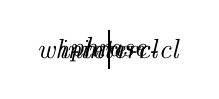
\begin{tikzpicture}[baseline=(root.base)]
        \Tree 	[.\node(root){\emph{phrase}};
                    [.\textsc{headedness}
                        \dots{}
                        [.\emph{headed-phrase}
                            \dots{}
                            \dots{}
                            [.\emph{head-fill-ph}
                                \dots{}
                                \dots{}
                                \node(wh-interr-cl){\emph{wh-interr-cl}};
                            ]
                        ]
                    ]
                    [.\textsc{clausality}
                        [.\emph{clause}
                            \node(interr-cl){\emph{interr-cl}};
                            \dots{}
                        ]
                        \emph{non-clause}
                    ]
                ]

            \draw (interr-cl.south) to (wh-interr-cl.north);

    \end{tikzpicture}
\z
%
\emph{head-fill-ph}, \emph{interr-cl}, and \emph{wh-interr-cl} are
abbreviations for \emph{head-filler-phrase}, \emph{interrogative-clause}, and
\emph{wh-interrogative-clause}, respectively. Other subtypes of
\emph{headed-phrase}  are \emph{head-complement-phrase} (for combinations of a
word and its complements) and \emph{head-subject-phrase} (for combinations of a
phrase and its subject), and other subtypes of \emph{head-filler-phrase}
include \emph{wh-relative-clause}. Again, all the types will be subject to
appropriate constraints. For example, \emph{headed-phrase} will be subject to a
constraint requiring it to have a head daughter with which it shares certain
properties. This system allows all sorts of generalizations to be captured.
Properties that are shared by all phrases can be captured by a constraint on
\emph{phrase}, properties that are shared by all headed-phrases by a constraint
on \emph{headed-phrase}, properties that are shared by all head-filler-phrases
by a constraint on \emph{head-fill-ph}, and so on.

Among other things, constraints on the various phrasal types provide
information about what daughters they have. However, they don’t say anything
about the order of the daughters. This is the province of a separate set of
constraints. Obviously, this is an area in which languages may differ.

An \gls{HPSG}\is{Head-Driven Phrase Structure Grammar} syntactic analysis is quite complex, especially compared with
Minimalism, for which, as we have noted, syntax is just a few very general
mechanisms. However, it is not as complex as the base component of an
\emph{Aspects}-style grammar \citep{Chomsky1965} nor as the kind of grammar
proposed within the earlier \gls{GPSG} framework \parencite{GazKlePulSag1985}
Both approaches involve many different rules for combinations of a head and its
complement, a set of rules for VPs, a set for PPs, and so on. Most \gls{HPSG}
work has a single \emph{head-complement-phrase} type with no subtypes. This
raises the question: when do we need to postulate a phrasal type? There are, of
course, various different kinds of head-complement-phrase, but there is no need
for any subtypes. A verb-phrase is just a head-complement-phrase headed by a
verb with certain properties stemming from its head, while a prepositional
phrase is just a head-complement-phrase headed by a preposition, again with
certain properties stemming from its head. We can say the following:

\begin{quote}

A phrasal type is necessary whenever some set of phrases have properties which
do not follow either from the more general types which they instantiate or from
the lexical items that they contain.

\end{quote}
%
This might lead one to wonder whether a \emph{wh-interrogative-clause} type is
necessary. One point to emphasize here is that a
\emph{wh}-interrogative-clause is not just a head-filler-phrase with a
\emph{wh}-phrase as the filler. The \emph{wh}-phrase must have the
immediately containing clause as its scope. This is unlike the situation in
languages with so-called partial \emph{wh}-movement. Consider, for example,
the following \ili{German} example from \citet{McDaniel1989}.

\ea\label{ex:borsley:4.6} German\\
    \gll    Was glaubt Hans [[ mit wem ] Jakob jetzt spricht ]?\\
            what believes Hans {} with whom {} Jakob now speaks {}\\
    \glt    \enquote*{What does Hans think Jacob is speaking to now?}
\z
%
Here the \emph{wh}-phrase is in the subordinate clause, but, as the
translation makes clear, the scope of the \emph{wh}-word \emph{wem} is
the whole sentence. It is also necessary to ensure that \ili{English}
\emph{wh}-interrogatives have a pre-subject auxiliary\is{auxiliaries} if and only if it is
main clause. It may be possible to capture these facts without postulating a
\emph{wh-interrogative-clause} type, but it is not easy.

At least this is not easy if phonologically empty elements are not freely
available. If such elements are freely available, it may well be possible to
attribute the facts to the properties of a phonologically empty head. This is
essentially the approach which is taken in Minimalism, in which
head-filler-phrases involve structures of the following form, where X is
C(omplementizer) or one of the elements that replaces it in work stemming from
\citet{Rizzi1997}, e.g. Force, Top(ic), Foc(us).

\ea\label{ex:borsley:4.7}
    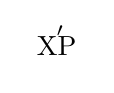
\begin{tikzpicture}[baseline=(xp.base)]

        \Tree 	[.\node(xp){XP};
                    YP
                    [.X$'$
                        X
                        ZP
                    ]
                ]

    \end{tikzpicture}
\z
%
The idea seems to be that the properties of X ensure that the specifier YP and
the complement ZP have the right properties. However, this idea never seems to
be developed in any detail. A detailed development would involve precise
lexical descriptions for the various empty heads. The sort of thing that is
necessary was developed in some early \gls{HPSG}\is{Head-Driven Phrase Structure Grammar} work. \textcite[Ch.\
5]{PolSag1994} outlined an approach to \ili{English} \isi{relative clauses} involving a
number of empty heads (an approach which was abandoned in \citealt{Sag1997}).
One of these heads has the following description:

\ea\label{ex:borsley:4.8}
     \small
     \avm[style=narrow]{
       [
        local & [ cat & [ head & [ mod n' [to-bind|rel \{ \1 \}]: [index & \1\\ restr & \3] ]\\
                          subcat & < [loc \4, inher | rel \{\1\}],\\
                                     s[ {\normalfont\itshape  fin, unmarked, } inher | slash \{\4\}]: \5 > ]\\
                  content & [ index & \1 \\ restr & \{\5 $\cup$ \3\}] ]\\
        \punk{nonlocal|to-bind|slash}{\{\4\}} ]
    }
\z
%
This interacts with certain phrase types to give a structure like
\REF{ex:borsley:4.7}. It is complex, but each component of it has a purpose. The \textsc{mod}
feature indicates that the maximal projection of this element modifies an N$ʹ$.
The \textsc{subcat} feature indicates that it combines with a specifier containing a
relative pronoun and a complement which is a finite clause with no
complementizer but a non-empty \textsc{slash} feature ensuring that it contains a
gap.\footnote{The \textsc{subcat} feature does work that is done by separate \textsc{subj} and
\textsc{comps} features in later work. \textsc{slash} does the work that is done in \gls{MGG} by
A$ʹ$-movement. For arguments that the \textsc{slash} mechanism provides a better account
of the phenomena, see \citet{Borsley2012}.} This feature also ensures that the
specifier has the properties in the value of \textsc{slash}. The \textsc{content} feature ensures
that the content of this element brings together the content of the modified N$ʹ$
and the relative clause. Various principles of \gls{HPSG}\is{Head-Driven Phrase Structure Grammar} ensure that the
combination of N$ʹ$ and relative clause has the content of the empty
head.\footnote{The \textsc{to-bind} features ensure that the \textsc{rel} and \textsc{slash} features do
not appear any higher in the tree than they should.} As noted above, this
approach has been abandoned, but it gives some idea of what is involved in
giving an explicit analysis of the kind of empty head that is central to the
Minimalist approach to head-filler-phrases.  It may be that Minimalist empty
heads will have simpler descriptions, but until such descriptions have been
developed, we cannot really know.

Within Minimalism it is not just head-filler-phrases whose properties have to
be derived in some way from a typically empty head. \ili{English} clauses without an
auxiliary have an empty T head, and \ili{English} nominal constituents without a
visible determiner have an empty D head. Thus, empty heads of various kinds are
central to Minimalism. This is a reflection of the fact noted earlier that the
syntax for Minimalism is just a few very general mechanisms. Minimalism is a
bit like a version of \gls{HPSG}\is{Head-Driven Phrase Structure Grammar} with just two phrase types, an External \isi{Merge}
type and an Internal \isi{Merge} type.\footnote{For further discussion of the
relation between the two approaches, see \citet{Muller2013}.} It follows that
the real work must be done by lexical elements and often by empty lexical
elements. Oddly, however, very little attention has been paid to the properties
of these elements.\footnote{\textcite[95, fn.\ 9]{Newmeyer2005} comments that
    \blockquote{\dots{} in no framework ever proposed by Chomsky has the
lexicon been as important as it is in the \glsunset{MP}\gls{MP} [\glsdesc{MP}].
Yet in no framework proposed by Chomsky have the properties of the lexicon been
as poorly investigated.}}

If empty elements are only postulated when there is compelling evidence for
them, there is no possibility of deriving the properties of different phrase
types from various invisible heads. Hence, a fairly complex syntax is more or
less inevitable. However, this need not be a problem for acquisition\is{language acquisition} if the
analysis is a fairly direct reflection of the observable data, as it is in
\gls{HPSG}.

As we have noted, a typical \gls{HPSG}\is{Head-Driven Phrase Structure Grammar} analysis will have a number of other
subtypes of \emph{head-filler-phrase}. Consider the following examples:

\ea\label{ex:borsley:4.9}
    the book [ which I am writing ]
\ex\label{ex:borsley:4.10}
    What an interesting book this is!
\ex\label{ex:borsley:4.11}
    The more I read, the more I understand.
\z
%
The bracketed material in \REF{ex:borsley:4.9} is a \emph{wh}-relative,
\REF{ex:borsley:4.10} is a \emph{wh}-exclamative, and \REF{ex:borsley:4.11} is what has
often been called a comparative correlative, a construction whose component
clauses have been called \emph{the}{}-clauses, e.g. in \citet{Borsley2011}. We
have three types of head-filler phrases each with various distinctive
properties. \emph{wh}-relatives may contain \emph{who} and \emph{which} but not
\emph{what}. \emph{wh}-exclamatives may only contain \emph{what}
\emph{a}(\emph{n}) or \emph{how}. Neither allows an auxiliary\is{auxiliaries} before the
subject. Finally, \emph{the}{}-clauses must contain \emph{the} and a
comparative word. The second clause but not the first may contain a pre-subject
auxiliary:

\ea\label{ex:borsley:4.12}
    \ea[]{The more I read, the more do I understand.}
    \ex[*]{The more do I read, the more I understand.}
    \z
\z
%
For \gls{HPSG}\is{Head-Driven Phrase Structure Grammar}, these facts can be handled by constraints on three additional
subtypes: \emph{wh-relative-clause}, \emph{wh-exclamative-clause}, and
\emph{the-clause}. See \citet{GinSag2000} and \citet{Sag2010}.

English also has \isi{relative clauses} with no visible relative pronoun. One might
propose that such \isi{relative clauses} have a phonologically empty relative
pronoun. But, as we have noted, \gls{HPSG}\is{Head-Driven Phrase Structure Grammar} only assumes such elements if there
is compelling evidence for them. In the absence of clear evidence for such an
element, this is just an ad hoc way of minimizing differences between
constructions. It is not difficult to provide an analysis which does not involve
an empty element. For \gls{HPSG}\is{Head-Driven Phrase Structure Grammar}, as
indicated earlier, \isi{relative clauses} have a feature \textsc{mod}, whose value
indicates what type of nominal phrase they modify. In a \emph{wh}-relative
clause, the value of \textsc{mod} is coindexed with the relative pronoun, as in
\REF{ex:borsley:4.13}:

\ea\label{ex:borsley:4.13}
    \begin{tikzpicture}[baseline,yshift=.75\baselineskip]
        \tikzset{level distance=50pt}
        \Tree 	[.\node(root){S\\{}[\textsc{mod} N$ʹ_{i}$]};
                    [.NP$i$ who ]
                    [.\node(s){S\\{}[\textsc{slash} \{NP$_i$\}]};
                        \edge [roof]; {I talked to}
                    ]
                ]
    \end{tikzpicture}
\z
%
The value of \textsc{slash} matches the filler and hence has the same index.\footnote{In
    a more complex example such as the following, where the relative pronoun is
    just part of the filler, the value of \textsc{slash} and the relative pronoun will
    have different indices:

\begin{exe}
    \exi{(i)} whose brother I talked to
\end{exe}} In a non-\emph{wh}-relative clause, the value of \textsc{mod} is coindexed
directly with the value of \textsc{slash}, as in \REF{ex:borsley:4.14}:

\ea\label{ex:borsley:4.14}
    \begin{tikzpicture}[baseline,yshift=.75\baselineskip]
        \tikzset{level distance=50pt}
        \Tree 	[.\node(root){S\\{}[\textsc{mod} N$ʹ_{i}$]};
                    [.NP I ]
                    [.\node(s){S\\{}[\textsc{slash} \{NP$_i$\}]};
                        \edge [roof]; {talked to}
                    ]
                ]

    \end{tikzpicture}
\z
%
This just requires a type \emph{non-wh-relative-clause} with an appropriate
constraint. See \citet{Sag1997} for discussion.

\section{HPSG and language variety}\label{sec-5:4}

An \gls{HPSG}\is{Head-Driven Phrase Structure Grammar} linguistic description involves types, features, and constraints,
and languages may differ in any of these areas. Some types, features, and
constraints will no doubt be universal, but others will be language-specific.
The more general types such as \emph{sign}, \emph{lexical-sign}, \emph{word},
\emph{lexeme}, and \emph{phrase} will probably occur in all languages with the
same features, but many others are likely to be language-specific or to have
language-specific features.

The types that are the value of various traditional features will differ from
language to language for obvious reasons. Languages differ in how many genders
and cases they have. Therefore, the features \textsc{gender} and \textsc{case} will differ in
what types they have as possible values. Languages may also differ in whether
or not they have these features. Only some languages have grammatical gender
and only some languages show morphological case\is{case!morphological case}. Of course, it is possible to
assume an abstract notion of \textsc{case} present in languages whether or not they have
morphological case, but this complicates the acquisition\is{language acquisition} task and necessitates
more complex innate machinery than would otherwise be needed. It is probably
not a position that would find favour outside MGG.\footnote{An abstract notion
of case (or Case) played an important role in the Government and Binding
framework, but it seems to be of little importance within Minimalism and it has
not been adopted outside \gls{MGG}.}

A question that arises here is whether languages have the same \textsc{gender} and \textsc{case}
feature if they have very different systems of values. Does a language with two
genders have the same \textsc{gender} feature as one with ten? Probably most researchers
would think that they do, but there is room for debate here. Of course,
questions like this are not peculiar to \gls{HPSG}\is{Head-Driven Phrase Structure Grammar} but arise in any theoretical
framework.

Within \gls{HPSG}\is{Head-Driven Phrase Structure Grammar}, whether or not a language has case is first and foremost a
question of whether the type \emph{noun} has \textsc{case} among its features. But there
is another question here: does the type \emph{adj} have \textsc{case} among its
features?  In some languages that have morphological case\is{case!morphological case} it is clearly a
property of adjectives as well as nouns. Consider e.g. \ili{German} or Arabic.
But in other languages with morphological case\is{case!morphological case}, it does not extend to
adjectives. The North-East Caucasian language \ili{Archi} is a relevant example
(see \citealt{BonBroChuCor2016} for discussion). Similar issues arise with
gender. If a language has gender, then the type \emph{noun} has \textsc{gender} among
its features, but it may or not be a feature of other types such as \emph{adj} or
\emph{verb}.

What about other features, e.g. the \textsc{head} feature? This will probably have a
large number of values (but not so many as it would have within Minimalism,
where numerous \enquote{functional} parts of speech have been postulated, e.g.\
Force, Top(ic)\is{topic}, and Foc(us)\is{focus} mentioned earlier). It is
likely, however, that there will be some variation from language to language.
Of course, just as there are questions about whether different languages can
have the same \textsc{gender} and \textsc{case} features,\is{case!case features} so there are questions about whether
they can have the same \emph{noun}, \emph{verb} and \emph{adjective} types.
\citet{Haspelmath2010} thinks not. However, most \gls{HPSG}\is{Head-Driven Phrase Structure Grammar} linguists seem to
assume they can, and this view is defended in \textcite[Sec.\ 2.2]{Muller2015}.

The questions that we have just highlighted arise in any theoretical framework.
However, it is possible to sidestep them in a framework that does not emphasize
formal analyses. \gls{HPSG}\is{Head-Driven Phrase Structure Grammar} with its
emphasis on detailed formal analysis makes this more or less impossible.

The lexicon is obviously a major area in which languages differ. For Minimalism
it is the only area in which differences may reside (a position often referred
to as the Borer--Chomsky Conjecture\is{Borer--Chomsky Conjecture}). This is an
automatic consequence of the fact, highlighted earlier, that all the real work
is done by lexical entries within Minimalism. This is not the case within
\gls{HPSG} given the important role of the system of phrasal types and
associated constraints. However, for \gls{HPSG}\is{Head-Driven Phrase Structure Grammar}, many differences between
languages are a lexical matter.\largerpage[1]

Most obviously, the same meaning will generally be associated with different
phonological properties in different languages. \ili{English} has \emph{dog} where
Welsh has \emph{ci} and \ili{Polish} has \emph{pies}. Clearly, however, there can be
other differences. A meaning may be associated with different \textsc{head} values in
different languages. Thus, for example, the \ili{Welsh} counterpart of the
modal verb \emph{must} is the noun \emph{rhaid} \enquote{necessity}, as in
\REF{ex:borsley:4.15}.

\ea\label{ex:borsley:4.15}\ili{Welsh}\\
    \gll Rhaid i mi adael.\\
            necessity to me leave.\Inf{}\\
    \glt    \enquote*{I must leave.}
\z
%
Clearly, such contrasts are common. The same meaning may also have different
selectional properties in different languages. It is clear that the selectional
properties of a word are predictable to a considerable extent from its
semantics. However, there is quite a lot of room for variation. Where one
language has an NP with one case, another language may have an NP with a
different case, or a PP. Similarly, where one language has a finite clause,
another may have a non-finite clause, or some kind of nominalized clause.
Within \gls{HPSG}\is{Head-Driven Phrase Structure Grammar}, what case subjects have is also commonly seen as a matter of
selection. In some languages, all subjects or all subjects of finite verbs may
have nominative\is{nominative case} case, but in other languages there are other possibilities.

Turning to syntax, we emphasized above that \gls{HPSG}\is{Head-Driven Phrase Structure Grammar} only postulates empty elements
when there is compelling evidence for them. This has obvious implications for
comparisons between languages. If empty elements are not freely available,
there is no possibility of saying that languages are much the same but look
different because elements that are overt in one are empty in others. It
follows that we should expect substantial differences between languages in this
area.

The central question here is: how far can languages vary in the phrasal types
that they employ and the constraints to which they are subject? Probably all
languages will have the type \emph{headed-phrase} and
\emph{head-complement-phrase} as one of its subtypes. Perhaps they will also
have the types \emph{head-subject-phrase} and \emph{head-filler-phrase}. But
this may not be the case. Moreover, if two languages have the same type, it may
well have different subtypes from language to language.

As noted above, it may be that all languages will have the type
\emph{head-filler-phrase}. But it is clear that languages will differ in what
subtypes of \emph{head-filler-phrase} they have. A \emph{wh}-in-situ language
will not have \emph{wh-interrogative-clause} among the subtypes of
\emph{head-filler-phrase}. Since \emph{wh}-interrogatives have the same
structure as ordinary clauses in such languages, they will probably have a type
\emph{wh-interrogative-clause} which is a subtype of
\emph{head-subject-phrase}, giving the following situation:

\ea\label{ex:borsley:4.16}
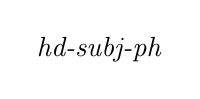
\begin{tikzpicture}[baseline=(hd.base), grow'=up]

        \Tree   [.\emph{wh-int-cl}
                    \node (hd) {\emph{hd-subj-ph}};
                    \emph{inter-cl}
                ]

    \end{tikzpicture}
\z
%
One might wonder here whether phrasal types that have different supertypes (and
are subject to different constraints) can really be viewed as the same type. I
will not try to decide this question.

As we noted above, another subtype of \emph{head-filler-phrase} in \ili{English} is
\emph{wh-relative-clause}. It seems, however, that most languages have relative
clauses with no sign of a fronted relative pronoun. One might propose that
relative clauses in such languages have a phonologically empty relative
pronoun. But, as emphasized above, this is not a move that would find favour in
\gls{HPSG}. In the absence of any concrete evidence for such an element, it is
just an ad hoc way of minimizing differences between languages. Thus, whereas
English has both a \emph{wh-relative-clause} type and a
\emph{non-wh-relative-clause} type, many languages seem to just have the
latter.

As also noted earlier, another subtype of \emph{head-filler-phrase} is required
to accommodate the two clauses in comparative correlatives such as the
following:

\ea\label{ex:borsley:4.17}
    The more I read, the more I understand.
\z
%
Other languages have broadly similar constructions.\footnote{This is noted by
    \citet[498]{denDikken2005b}, who claims that the construction is
    \enquote{analyzable in keeping with the principles and \isi{parameters} of
    \glsunset{UG}\gls{UG}}.  However, he does not provide an analysis. See
\textcite{AbeBor2008} for critical discussion.} Consider e.g.\ \ili{French} and
Spanish:

\ea\label{ex:borsley:4.18}\ili{French}\\
    \gll Plus je lis, plus je comprend.\\
            more I read more I understand\\
    \glt    \enquote*{The more I read, the more I understand.}
\ex \label{ex:borsley:4.19}\ili{Spanish}\\
    \gll Cuanto más leo, (tanto) más entiendo.\\
            how.much more I.read that.much more I.understand\\
    \glt    \enquote*{The more I read, the more I understand.}
\z
%
In the \ili{French} construction, there is no counterpart of \emph{the}, while
the \ili{Spanish} construction has two different elements, \emph{cuanto} ‘how-much’
and \emph{tanto} ‘that-much’, the latter being optional. Maybe both languages
will have the same subtype of \emph{head-filler-phrase} (though a different
name might be appropriate) but the subtype will be subject to somewhat
different constraints. In some languages, the second clause need not be a
head-filler-phrase. One such language is \ili{Dutch}, with examples like the
following:

\ea\label{ex:borsley:4.20}Dutch\\
    \gll Des te meer je leest, je begrijpt des te minder.\\
            the.\Gen{} \textsc{te} more you read you understand the.\Gen{} \textsc{te} less\\
    \glt    \enquote*{The more you read the more you understand.}
\z
%
Thus, broadly similar constructions may differ in important ways and pose
various analytic challenges.\footnote{For further discussion and analyses of
the \ili{French} and \ili{Spanish} constructions, see
\textcite{AbeBorEsp2006,AbeBor2008}.}

As noted above, the type \emph{headed-phrase} has a number of subtypes. In
addition to those mentioned, there is a \emph{head-adjunct-phrase} type
required for adjective and nominal combinations such as \emph{old} \emph{men}
and verb-phrase and adverb combinations such as \emph{walk} \emph{slowly}. It
may be that another subtype is necessary for verb-initial\is{verb-initial constituent order} clauses such as
\REF{ex:borsley:4.21}.

\ea\label{ex:borsley:4.21}
    Is Kim a linguist?
\z
%
\gls{HPSG} rejects the view that all branching is binary and generally assumes
a ternary branching analysis for such clauses.\footnote{The arguments for the
binary branching restriction have never been very persuasive, see e.g.\
\citet[112--116]{CulJac2005}.} An obvious approach is one in which both the
subject and the complement are sisters of the verb, as in the following
structure:

\ea\label{ex:borsley:4.22}
    \begin{tikzpicture}[baseline=(root.base)]

        \tikzset{frontier/.style={distance from root=100pt}}

        \Tree
            [.\node(root){S};
                [.\node[minimum size=2cm](V){V\\
                    \avm{[ subj & <\1>\\ comps & <\2>]}};
                    is
                ]
                [.{\avm{\1} NP} Kim ]
                [.{\avm{\2} NP} \edge[roof]; {a linguist} ]
            ]

    \end{tikzpicture}
\z
%
This approach requires an additional subtype of \emph{headed-phrase}, which can
be called \emph{head-subject-complement-phrase}, with an appropriate
constraint. But there is an alternative approach to verb-initial\is{verb-initial constituent order} clauses, in
which the verb takes two complements and no subject, giving a structure like
the following:

\ea\label{ex:borsley:4.23}
    \begin{tikzpicture}[baseline=(root.base)]

        \tikzset{frontier/.style={distance from root=100pt}}

        \Tree
            [.\node(root){S};
                [.\node(V){V\\
                    \avm{[subj & < \1 >\\comps & < \2 >]}};
                    is
                ]
                [.{\avm{\1} NP} Kim ]
                [.{\avm{\2} NP} \edge[roof]; {a linguist} ]
            ]

    \end{tikzpicture}
\z
%
This is an ordinary head--complement structure, but it requires special lexical
descriptions for auxiliary\is{auxiliaries} verbs. These can be derived from the standard
lexical descriptions by a lexical rule. The first of these approaches is
adopted in \citet[36]{GinSag2000}, while the second approach is assumed in
\citet[410]{SagWasBen2003}. One possibility is that the two approaches are
relevant to different languages. Thus, \citet{Borsley1995} argues that the
first approach is right for verb-initial\is{verb-initial constituent order} clauses in Syrian Arabic, while the
second is appropriate for verb-initial\is{verb-initial constituent order} clauses in Welsh.

One further point to note here is that a structure in which both the subject
and the complement (or complements) are sisters of the verb is potentially
relevant not just to clauses in which verb and complement(s) are separated by
the subject but also to clauses in which they are adjacent. That is, there may
be SVO or SOV clauses in which there is a flat structure and no VP. Thus,
\citet{Borsley2016} argues that such an analysis is appropriate for SOV clauses
in \ili{Archi}. On this analysis, \REF{ex:borsley:4.24} has the schematic analysis in
\REF{ex:borsley:4.25}.

\ea\label{ex:borsley:4.24}Archi\\
    \sn
    \gll zari noˤš darcʹ-li-r-ši e‹b›tʹni.\\
            \Fsg.\Erg{} horse.\Iii{}[\Sg.\Abs{}] post-\Obl.\Sg{}-\Cont-\All{} ‹\Iii.\Sg›.tie.\Pfv{}\\
    \glt    \enquote*{I tied the horse to the post.}
\z

\ea\label{ex:borsley:4.25}
    \begin{tikzpicture}[baseline=(root.base)]

        \tikzset{frontier/.style={distance from root=80pt}}

        \Tree
            [.\node(root){S};
                [.{NP\\{}[\textsc{case} \Erg{}]} zari ]
                [.{NP\\{}[\textsc{case} \Abs{}]} noˤš ]
                [.{NP\\{}[\textsc{case} \Obl{}]} darcʹ-li-r-ši ]
                [.{V} e‹b›tʹni ]
            ]

    \end{tikzpicture}
\z
%
Thus, the fact that V and O are normally adjacent in some language does not
necessarily mean that they form a VP constituent.

A more general point that we should make here is that it is important not to
assume too quickly that something that looks rather like an \ili{English}
realization of a specific phrase type is just another realization of that type.
For \gls{HPSG}\is{Head-Driven Phrase Structure Grammar}, \ili{English} subject-initial clauses are realizations of a
\emph{head-subject-phrase} type. \ili{Arabic} also has subject-initial clauses,
e.g. the following:

\ea\label{ex:borsley:4.26}\ili{Arabic}\\
    \gll T-tullaab-u qaabaluu {/} \llap{*}qaabala Aħmad-a.\\
            the-students-\Nom{} met.\Tpl.\M{} {} met.\Tsg.\M{} Ahmad-\Acc{}\\
    \glt    \enquote*{The students met Ahmad.}
\z
%
One might assume that these are head-subject-phrases. However, another
possibility is that they are verb-initial\is{verb-initial constituent order} clauses with an initial NP \isi{topic} and
hence head-filler-phrases. This might seem dubious initially. The verb in a
subject-initial clause shows full agreement for person, gender, and
number.\is{agreement!subject agreement}\is{agreement!number agreement} The
situation is different in verb-initial\is{verb-initial constituent order} clauses, as the following shows:

\ea\label{ex:borsley:4.27}\ili{Arabic}\\
    \gll qaabala {/ } \llap{*}qaabaluu T-tullaab-u Aħmad-a.\\
            met.\Tsg.\M{} {} met.\Tpl.\M{} the-students-\Nom{} Ahmad-\Acc{}\\
    \glt    \enquote*{The students met Ahmad.}
\z
%
Here, we have partial agreement, \isi{agreement} for person and gender but not
number. This might be seen as evidence against the idea that subject-initial
clauses are clauses with an initial \isi{topic}. Consider, however, an example with
an initial \isi{topic} interpreted as subject of a subordinate clause:

\ea\label{ex:borsley:4.28}\ili{Arabic}\\
    \gll T-tullaab-u ʔiqtaraħtu {[} ʔan yušaarikuu {/ } \llap{*}yušaarika fii l-musaabaqat-i ].\\
            the-students-\Nom{} suggested.\Fsg.\M{} {} that participate.\Tpl.\M{} {} participate.\Tsg.\M{} in the-competition-\Gen{}\\
    \glt    \enquote*{The students I suggested participate in the competition.}
\z
%
The complementizer\is{complementizers} \emph{ʔan} only introduces verb-initial\is{verb-initial constituent order} clauses. Hence the
subordinate clause here is a verb-initial\is{verb-initial constituent order} clause, but it shows full
\isi{agreement}.  This seems surprising. However, the problem disappears if we
assume that the clause has a null pronominal subject coindexed with a preceding
topic. Null subject sentences,\is{null subjects} which I assume have a null pronominal subject,
show full agreement.\is{agreement!subject agreement} Thus, the following can only have the meaning indicated
and cannot mean that they met Ahmad:

\ea\label{ex:borsley:4.29}\ili{Arabic}\\
       \gll laqad    qaabala    Aħmad-a.\\
            indeed met.\Tsg.\M{} Ahmad-\Acc{}\\
    \glt    \enquote*{He met Ahmad.}
\z
%
Essentially the same analysis can be applied to \REF{ex:borsley:4.26}. That is, it
too can be analysed as involving an initial \isi{topic} coindexed with a null
pronominal subject. If this is right, \REF{ex:borsley:4.26} is not a
head-subject-phrase but a head-filler-phrase.\footnote{This argument
is taken from \citet{AloBor2013}.} Maybe \ili{Arabic} has some other kinds of
head-subject-phrase or maybe it has no head-subject-phrases at all.

We should now say something about word order. For \gls{HPSG}\is{Head-Driven Phrase Structure Grammar}, as for some other
frameworks, some word order differences between languages are not very
important. We noted earlier that constraints on the various phrasal types
provide information about what daughters they have, but say nothing about the
order of the daughters, which is the province of a separate set of constraints.
It follows that head-initial and head-final languages may have
head-complement-phrases that are identical apart from word order. This
contrasts with the situation in \citegen{Kayne1994} antisymmetry version of
\gls{MGG} in which complement-head order is the product of a \isi{movement} process
and hence more complex than head-complement order. The \gls{HPSG}\is{Head-Driven Phrase Structure Grammar} position is more
like that of versions of \gls{MGG} that assume a directionality parameter.
However, unlike such approaches, \gls{HPSG}\is{Head-Driven Phrase Structure Grammar} does not assume that a language will
linearize all head-complement structures in the same way. Hence, there is no
problem with a language like \ili{Finnish}, which has verb-object order but
postpositions, or a language like \ili{Persian}, which has object-verb order but
prepositions. Such languages will have two different linear precedence
constraints, while languages which order all head-complement structures in the
same way will have just one. Hence the latter are simpler in this area, and
this makes it unsurprising that they are more common.\footnote{Essentially this
point was made by \citet{FodCra1990} in a discussion focusing on the
earlier \gls{GPSG} framework.}

The fact just highlighted means that SVO and SOV languages may have VPs
licensed by the same \emph{head-complement-phrase} type. VSO languages are
different if they have either of the analyses in \REF{ex:borsley:4.22} and
\REF{ex:borsley:4.23}. (On the analysis in \REF{ex:borsley:4.23} the clause is a
head-complement-phrase but it is not an ordinary VP.) However, there is an
alternative approach which might be taken to VSO clauses. Much work in
\gls{HPSG} has proposed that linear order is a reflection not of the
constituent structure of an expression but of a separate system of order
domains \parencite[see][]{Reape1992,Muller1996,Kathol2000}.  Within this
approach, the constituent structure of an expression is encoded as the value of
a \textsc{dtrs (daughters)} feature and the order domain as the value of a \textsc{dom(ain)}
feature. Adopting it, one might propose that the \ili{Welsh} VSO sentence in
\REF{ex:borsley:4.30} has the schematic analysis in \REF{ex:borsley:4.31}.

\ea\label{ex:borsley:4.30}\ili{Welsh}\\
    \gll Gwelodd      Emrys  y    ddraig.\\
            see.\Pst.\Tsg{} Emrys the dragon\\
    \glt    \enquote*{Emrys saw the dragon.}
\z

\ea\label{ex:borsley:4.31}
    \avm{
      [synsem & S\\
       dtrs & < \normalfont\itshape !{\ob}!Emrys!{\cb}!,~!{\ob}!gwelodd y ddraig!{\cb}!>\\
       dom  & < \normalfont\itshape !{\ob}!gwelodd!{\cb}!,~!{\ob}!Emrys!{\cb}!,~!{\ob}!y ddraig!{\cb}!>
      ]
    }
\z
%
On this analysis \ili{Welsh} has finite VPs just like \ili{English}. One could
propose essentially the same analysis for verb-initial\is{verb-initial constituent order} clauses in a language in
which the existence of finite VPs is uncontroversial, e.g.\ \ili{English}. In
\citet{Borsley2006}, I argue against an analysis of this kind for \ili{Welsh}
and in favour of an analysis of the kind in \REF{ex:borsley:4.23}. It could be,
however, that the approach in \REF{ex:borsley:4.31} is appropriate for other VSO
languages or for verb-initial\is{verb-initial constituent order} clauses in some language of other types.

Even if order domains are not appropriate for \ili{Welsh} VSO clauses, they
provide a plausible approach to various other phenomena. For example, they
might be used to provide an account of extraposed \isi{relative clauses}, such as
\REF{ex:borsley:4.32}, which might have the analysis in \REF{ex:borsley:4.33}.

\ea\label{ex:borsley:4.32}
    A man came in who looked like Chomsky.
\ex \label{ex:borsley:4.33}
    \avm{
      [synsem & S\\
       dtrs & < \normalfont\itshape !{\ob}!a man who looked like Chomsky!{\cb}!,~!{\ob}!came in!{\cb}!>\\
       dom  & < \normalfont\itshape !{\ob}!a man!{\cb}!,~!{\ob}!came in!{\cb}!,~!{\ob}!who looked like Chomsky!{\cb}!>
      ]
    }
\z
%
Alternatively, however, one might assume that such examples are rather like
head-filler-phrases but with the filler constituent on the right.

Order domains seem most plausible as an approach to the sorts of discontinuity
that are found in so-called nonconfigurational languages such as
\ili{Warlpiri}.\footnote{ \textrm{See e.g. \citet{DonohueSag1999}.}} However, they
may well have a role to play in more familiar languages. Exactly how much of a
role they play in syntax is an unresolved matter.

The preceding remarks illustrate the fact that there are often a number of
plausible approaches to some syntactic phenomenon. This means that it is not
easy to know what the right analysis is and that it is hard to be confident
that one has the right analysis for any phenomenon. Deciding on an analysis is
somewhat easier if you subscribe to a theoretical framework which limits the
range of possible analyses, e.g. by excluding more than binary branching or by
insisting with \citet{Kayne1994} that there is a universal
specifier-head-complement order. The first restriction is generally accepted
within Minimalism, and the second quite widely accepted. Outside Minimalism,
however, the view is that there is little motivation for them. Whatever
framework one subscribes to, there are many unresolved issues, even in a
language like \ili{English}, which has been studied by numerous syntacticians over
many decades. Naturally, there are many more such issues in languages which
have a lot less attention. All this means that there is little basis for strong
claims about language universals or the extent to which languages may vary.

\section{Further discussion}\label{sec-5:5}

The previous section ended on what might be seen as a negative note. It seems
to me that this is a realistic assessment, but some researchers have painted a
much rosier picture. Not so long ago, \citet{Baker2001} commented that:
\blockquote[{\citealt[50]{Baker2001}}]{We are approaching the stage where we can
imagine producing the complete list of linguistic \isi{parameters}, just as
Mendeleyev produced the (virtually) complete list of natural chemical
elements}. It is not clear that many would share this optimism now. In any
event, I do not see how this could be justified. We could only be confident
about any set of proposals about \isi{parameters} if we had detailed formal analyses
for a wide range of languages employing them. There are of course proposals
about many phenomena in many languages, but the detail and precision is
generally lacking. Thus, \citet[535]{CulJac2005} comment that \enquote{much of
the fine detail of traditional constructions has ceased to garner attention}.

The limited nature of our knowledge is sometimes recognized within \gls{MGG}.
Thus, \textcite[382, fn.\ 22]{Chomsky1995} remarks that: \blockquote{\dots{}
we still have no good phrase structure theory for such simple matters as
attributive adjectives, \isi{relative clauses}, and adjuncts of different types}.  No
doubt there has been some progress since 1995, but there are clearly still many
unresolved issues about these phenomena both in \ili{English} and in other
languages. Obviously, other languages are very important here.  The vast
majority of languages have had a fraction of the attention that has been
lavished on \ili{English}. If other languages were broadly similar to \ili{English}, this
might not matter, but it is hard to deny that there are major differences. I
highlighted a number of differences in the previous section, but it may be that
languages can differ even more fundamentally from \ili{English}.
\citet{KoeMich2014} argue that \ili{Oneida} has no standard syntactic
features. In similar vein, \textcite{Gil2005,Gil2009} argues that \ili{Riau
Indonesian} has no parts of speech, almost no function words, and virtually no
morphology.\footnote{But see \citet{Yoder2010} some critical discussion.} It is
possible that someone will be able to show that these languages are less
different from familiar languages than they appear, but at present they suggest
that language variety is rather greater than is often suggested. We may
eventually have a firm basis for claims about language universals and the
extent to which languages may vary, but currently this seems a long way off. So
at least it seems to most people within \gls{HPSG}.\largerpage

Another feature of \gls{HPSG}\is{Head-Driven Phrase Structure Grammar}, alluded to above, which is very relevant in the
present context is the emphasis on the importance of firm empirical foundations
in the form of detailed formal analyses of the kind advocated by
\citeauthor{Chomsky1957} in \emph{Syntactic Structures}. Whereas \gls{MGG}
typically offers sketches of analyses which might be fleshed out one day,
\gls{HPSG} commonly provides detailed analyses which can be set out in an
appendix. As noted above, \citet{GinSag2000}, which sets out its analysis of
\ili{English} interrogatives in a 50 page appendix, is a notable example.
Arguably one can only be fully confident that a complex analysis works if it is
incorporated into a computer implementation. Hence, computer implementations of
\gls{HPSG} analyses are quite common. Particularly important here is the
CoreGram project reported in \citet{Muller2015}, which seeks to develop
computational grammars for a diverse range of languages. Among other things,
this permits a fairly precise measure of how similar or how different grammars
are, in terms of shared constraints or shared lines of code. Analyses that are
not implemented or are only partly implemented can be very valuable, but it
seems likely that implemented analyses will be increasingly important in
syntax, and that includes comparative syntax.

A further important feature of \gls{HPSG}\is{Head-Driven Phrase Structure Grammar}, highlighted above, is its avoidance
of abstract analyses with elements or properties for which there is no clear
evidence in the data. There may be real evidence for such elements and
properties, but research in \gls{HPSG}\is{Head-Driven Phrase Structure Grammar} suggests that they are generally
unnecessary.  For example \citet{GinSag2000} can be seen among other things as
a demonstration that \ili{English} interrogatives do not require either
movement processes or abstract structures, and much the same can be said of
\citet{Sag1997} and \ili{English} \isi{relative clauses}. As was emphasized above,
grammars that are quite closely related to the observable data pose less
of a problem for acquisition\is{language acquisition} than grammars that are more abstract and hence
create less need for some innate apparatus. This is surely something that
anyone should view as a good thing.\footnote{One might think that the acquisition\is{language acquisition}
    task is fairly simple if languages have essentially the same structures
    differing only in what is and what is not visible. But this seems doubtful.
    As \citet[765]{Fodor2001} puts it, \blockquote{It is clear now that even if
        the structural scaffolding of sentences is everywhere fixed and the
        same, any particular sentence may be highly ambiguous with respect to
        how its words are attached to that scaffolding.} Essentially, the more
        complex the structure of sentences is and the more invisible material
    it may contain, the harder it is for the learner to determine where
anything is. As \citet[763]{Fodor2001} comments, on this view, \enquote{natural
language design is extremely cruel to children}.}

As noted above, this outlook on grammar construction entails that the fact that
many languages have some element or property should not be seen as evidence
that they all do. Many languages have case and many languages have
\isi{agreement}, but it does not follow that they all do. In much the same way,
many birds fly, but it does not follow that they all do, even those such as
ostriches and penguins which never seem to get off the ground. As
\citet[25]{Muller2015} puts it, \enquote{grammars should be motivated on a
    language-specific basis.} Does this mean that other languages are
    irrelevant when one is investigating a specific language?  Clearly not. As
    Müller also puts it, \blockquote[{\citealt[43]{Muller2015}}][.]{In
        situations where more than one analysis would be compatible with a
    given dataset for language X, the evidence from language Y with similar
constructs is most welcome and can be used as evidence in favor of one of the
two analyses for language X} In practice, any linguist working on a new
language will use apparently similar phenomena in other languages as a starting
point. It is important, however, to recognize that apparently similar phenomena
may turn out on careful investigation to be significantly different. I made
this point in the last section in connection with subject-initial clauses in
Modern Standard Arabic.  \ili{Arabic} comparatives provide a rather different
illustration.

Like many languages, Modern Standard Arabic\il{Modern Standard
Arabic|see{Arabic}} has simple comparatives with a comparative form of an
adjective and complex comparatives with two separate elements:


\ea\label{ex:borsley:4.34}\ili{Arabic}
    \ea\label{ex:borsley:4.34a}
        \gll    heya    ʔaTwal-u           min    xalid-in\\
                she taller.\F.\Sg.\Nom{} from Khalid-\Gen{}\\
        \glt    \enquote*{She is taller than Khalid.}
    \ex\label{ex:borsley:4.34b}
        \gll    ʔanaa        ʔakthar-u    thakaʔ-an          min    ali-in\\
                \Fsg.\M{} more-\Nom{} intelligence-\Acc{} from Ali-\Gen{}\\
        \glt    \enquote*{I am more intelligent than Ali.}
    \z
\z
%
Superficially, these examples are much like their \ili{English} translations
and like simple and complex comparatives in many other languages. However, as
the gloss of \REF{ex:borsley:4.34b} makes clear, \emph{thakaʔ-an} is not an
adjective like \emph{intelligent}, but what can be called an adjectival noun
(with accusative\is{accusative case} case). This might seem like a minor, unimportant difference.
However, there is evidence that it is an important matter, reflecting the fact
that \ili{Arabic} complex comparatives are a quite different construction from
the complex comparatives of many other languages. The most important evidence
comes from the fact that the construction can contain not just adjectival nouns
but also ordinary nouns:

\ea\label{ex:borsley:4.35}\ili{Arabic}\\
    \gll ʔanaa        ʔakthar-u    maal-an      min    ali-in\\
            \Fsg.\M{} more-\Nom{} money.\Acc{} from Ali-\Gen{}\\
    \glt    \enquote*{I have more money than Ali.}
\z
%
It is fairly clear that \REF{ex:borsley:4.34b} involves the same comparative
construction as \REF{ex:borsley:4.35}. To reflect this, it could be translated as
\enquote{I have more intelligence than Ali}. The comparative construction in
\REF{ex:borsley:4.34b} and \REF{ex:borsley:4.35} is quite like what is called the
adjectival construct construction, illustrated in \REF{ex:borsley:4.36}.

\ea\label{ex:borsley:4.36}\ili{Arabic}\\
    \gll ’anta    azīm-u        l-hazz-I\\
            you    great-\Nom{}    the-fortune-\Gen{}\\
    \glt    \enquote*{You have great luck.}, \enquote*{You are very lucky.}
\z
%
The nominal in the adjectival construct is genitive\is{genitive case} and definite whereas that
in the comparative construction is accusative\is{accusative case} and indefinite. However, in both
cases, we have an adjective with an extra nominal complement, and in both, we
have what can be called a possessive interpretation. Thus, the construction in
\REF{ex:borsley:4.34b} is very different from its counterpart in \ili{English} and
other languages.\footnote{See \citet{AlsArnBor2017} for detailed discussion of
the facts.}

Thus, phenomena that look familiar may turn out to be rather exotic. Of course
it may also turn out that what look like unfamiliar phenomena are not so very
different from phenomena one is familiar with. All this just means that syntax
is complex and that it is not easy to get a clear picture of the syntax of any
language.

\section{Concluding remarks}\label{sec-5:conclusions}

I have argued in the preceding pages that \gls{HPSG}\is{Head-Driven Phrase Structure Grammar} is a framework that can
make a major contribution to the comparative syntax. It has a number of
features that are important here. The first is its emphasis on detailed formal
analyses of the kind envisaged in \emph{Syntactic Structures}, often
incorporated into a computer implementation. This means that the framework
provides firmer foundations than some other approaches for claims about
individual languages and ultimately about language in general. Secondly, it is
cautious about advancing strong claims about the universal properties of
language and the extent of linguistic variation. Some may feel that bold
conjectures act as a stimulus for research, but it is not clear that they are
any more effective in this regard than sober and cautious assessments of what
is and is not known. Finally, there is the avoidance of abstract analyses with
tenuous links to the observable data. As I have emphasized, this makes the
acquisition problem less difficult than it would be if grammars were more
abstract and hence creates less need for innate apparatus. For these reasons,
\gls{HPSG} has a lot to offer for anyone interested in comparative syntax and
looking for a suitable theoretical framework.\largerpage

\printchapterglossary{}

\section*{Acknowledgements}

I am grateful to Stefan Müller, Fritz Newmeyer, Maggie Tallerman and two
anonymous referees for their comments on an earlier version of this paper. Of
course I alone am responsible for what appears here.

{\sloppy
\printbibliography[heading=subbibliography,notkeyword=this]
}

\end{document}


